\documentclass[8pt]{beamer}
\usepackage{tikz}
\usepackage[utf8]{inputenc}


%Information to be included in the title page:
\title{Interleaved Quadrature and Optimization for Planning in Continuous State-Action Space}
\author{Nishad Gothoskar}
\institute{LIS}
\date{July 27 2018}
 
\begin{document}
 
\frame{\titlepage}
 
\begin{frame}
\frametitle{Value Function: Discrete vs. Continuous}
Discrete
\begin{equation*}    % <--- deleted empty lines
        V^{\pi}(s) = \max_{a \in A} \Big[\sum_{s' \in S} p_{s'|s,a}(s'|s,a)\big(R(s'|s,a) + \gamma V^{\pi}(s')\big) \Big]
\end{equation*}
Continuous
\begin{equation*}    % <--- deleted empty lines
        V^{\pi}(s) = \max_{a \in A} \int_{s' \in S} p_{s'|s,a}(s'|s,a)\big(R(s'|s,a) + \gamma^{\Delta t}V^{\pi}(s')\big) \ \textup{d}s'
\end{equation*}
\newline
In the continuous setting, a value update consists of a maximation over an integral.  More specifically, this is a maximization in a continuous action space and an integral of the product of a continuous state space value function and transition model.
\end{frame}

\begin{frame}
\frametitle{Gaussian Process in RL}
\begin{figure}
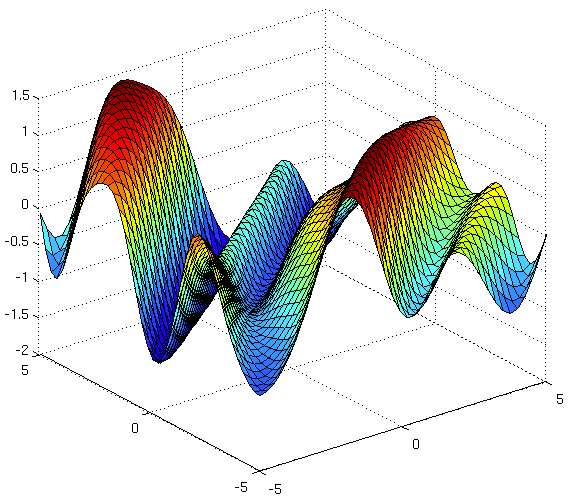
\includegraphics[scale=0.15]{gp}
\end{figure}
As opposed to discretizing the state space, we use a Gaussian Process to model the value function across the entire domain. Previous work in [1][2][3] has presented approaches to using GPs as value functions and learning a policy for a simple reinforcement learning problem (mountain car/swinging pendulum). There are many added complexities when working in larger state spaces and with complex dynamics models.
\newline  \newline

\end{frame}

\begin{frame}
\frametitle{Background}
Gaussian processes output a distribution of value at a state, which allows us to explicitly model our uncertainty about its value.
\begin{equation*}    % <--- deleted empty lines
	y^{*}|\bold{y} \sim \mathcal{N}(K_{*}K^{-1}\bold{y}, K_{**} - K_{*}K^{-1}K_{*}^{T})
\end{equation*}

In addition, when using Gaussian kernels for the GP and assuming Gaussian or mixture of Gaussian transition models, the following integral will have a closed form solution (mean and variance). By taking this into account when designing an action selection policy, we can tune the "hyperparameters" of our final policy.
\begin{equation*}    % <--- deleted empty lines
        \int_{s' \in S} p_{s'|s,a}(s'|s,a)\big(R(s'|s,a) + \gamma^{\Delta t}V^{\pi}(s')\big) \ \textup{d}s'
\end{equation*}
\end{frame}

\begin{frame}
\frametitle{Problem Statement}
In this work, we present a framework for planning in stochastic continuous state-action spaces. We use a GP to model the value across the entirety of the state space. Using this model to actively select states to update in each iteration, therefore extending previous methods to be feasible in large high-dimensional state spaces. In addition, using the previously mentioned quadrature techniques paired with a learned transition model, we estimate the value and uncertainty of taking certain actions, aiding in the action selection procedure. We show this method of active state selection and interleaved quadrature and optimization allows us to learn robust policies efficiently. We evaluate these policies with both a point robot in simulation and a block pushing scenario on the PR2.
\end{frame}

\begin{frame}
\frametitle{Current Method}
Our current approach
\end{frame}
 
\end{document}

